\documentclass[11pt]{article}
\usepackage[pdftex]{graphicx}
\usepackage{amsmath}

\title{A Survey of Parallelization of Kalman Filters}
\author{
       Brian J Gravelle 
}
\date{\today}


\begin{document}
\maketitle

\begin{abstract}
Kalman Filters have been an important aspect of many computer systems since they were first developed in the 1960s. Many of these applications require real-time speeds which has necessitated the parallelization of the Kalman filter from early in its development. This survey explores efforts to accelerate the algorithm with parallel techniques over the last 30 years  and discusses of the domains to which those parallelizations were applied. Many of the techniques are highly specialized to a particular domain so special care is given to how the parallelizations could be applied to different areas or are restricted to a specific application. Additionally, some discussion of future research is provided.
\end{abstract}

\section{Introduction}
Since their inception in 1960 Kalman filters have been heavily used for the estimation of states in dynamic systems. These filters have numerous applications especially in tracking various objects; they have been used to track object in conjunction with computer vision, radar tracking for airplanes and ships, vehicle and missile guidance systems, orbit calculation for satillites, and particles in HEP. Additionally, they have been used for demographic and economic studies, industrial process control, climate science, and geological surveys. Often these applications, the tracking ones especially, require real-time performance, pushing the performance demands of Kalman filtering.

At first the filtering was done primarily using customized circuits, each designed for the specific application to match the number of states in use. As modern computers developed, new opportunities for flexibility and improved performance were discovered. In many cases parallelism at different levels features in the performance enhancement of the Kalman filter. This survey reviews some of the implementations and applications of parallel Kalman filters.

The rest of the paper is not organized but is as follows: Section 2 covers background on the Kalman filter; Section 3 discusses some early implementations of parallel Kalman filters; Section 4 presents more recent implementations and applications; Section 5 talks about Kalman filters parallelized over distributed sensor networks; Section 6 is about FPGA implementations; and Section 7 concludes. I sincerely apologize for the case study of bad writing that this paper is.


\section{Background}
Kalman filters \cite{kalman1960new} were originally presented in 1960 to provide a solution to filtering and prediction problems in dynamic systems. In particular, the results targeted signals involved in communication and control systems. Since then, the Kalman filter has been applied to many dynamic systems in fields including physics, signal processing, economics, and others. In this section, we present some background information to enable the reader to better understand the rest of the survey. Interested readers are directed to the following sources: \cite{blackman1986multiple, welch1995introduction, budhiraja2007survey, kalman1960new}.

The Kalman filter is used to estimate the state of some dynamic system based on measurements, models, and associated errors of that system. This information is combined into a set of matrices that represent the whole system (Table \ref{mats}). The sizes of the matrices are based on the number of states in the system model ($n$) and the number of states measured in each time step ($m$). While some applications have larger state sizes, most require only a small number of states, resulting in matrices that are at the largest 20x20. In addition to the matrices there are also two vectors; $x$ of length $n$ that holds the estimated state and $y$ of length m for the current measurements.

\begin{table}
\caption{List of matrices involved in the Kalman filter.} 
\label{mats}
\centering
\begin{tabular}{||c c c||} 
\hline
Name & Description & dimensions \\ [0.5ex] 
\hline\hline
A & system dynamics & $nxn$\\
\hline
C or H & measurement matrix & $mxn$\\
\hline
Q & process (system) noise & $nxn$\\
\hline
R & measurement noise & $mxm$\\
\hline
P & error covariance & $nxn$\\
\hline
K & Kalman gain & $nxm$\\
\hline
\end{tabular}
\end{table}

At each time step the predicted state and the most recent measurement are compared and these values, combined with the error matrices are used to predict the next state. This prediction is based on weighting the measurement and model (expressed in the Kalman gain) and emphasizing one over the other based on error values. The accuracy of the Kalman filter relies heavily of the accuracy of the error and covariance matrices since these are integral in determining the Kalman gain with each step.

The Kalman equations are shown in Equations 1 - 5. Equations 1 and 2 are the predict portion, estimating the next state based on past data. Equations 3 - 5 and the correct section, updating the estimated state and Kalman gain based on the measurement and predicted state. There are additional versions such as the Extended Kalman Filter that implement improvements such as time variant error functions, or other changes to improve performance or accuracy.

\begin{equation}
\hat{x}_{new} = A\hat{x}
\end{equation}

\begin{equation}
P=APA^T+Q
\end{equation}

\begin{equation}
K = PC^T(CPC^T+R)^{-1}
\end{equation}

\begin{equation}
\hat{x}=\hat{x}_{new} + K(y-C\hat{x}_{new})
\end{equation}

\begin{equation}
P=(I-KC)P
\end{equation}

\section{Early Work}
Since the kalman filter has been around for so long, they have been the subject of many research projects seeking to improve the performance and/or accuracy. Two of the early results are discussed in this section. Both works are intended for Multiple Target Tracking of planes, satellites, or other rapidly moving targets.

\subsection{Circuit Parallelization}
In \cite{Shaffer:1987:IPE:42040.42101}, Shaffer presents a circuit design for an extended Kalman filter. While this work is a hardware implementation rather than software, it still applies the theoretical concepts and parallel patterns that are common in modern parallel software. In particular, Shaffer uses a pipeline pattern to take advantage of the concurrency of the algorithm and streaming nature of the data. Figure \ref{fig:shaffer} shows the data flow diagram of the system.

\begin{figure}
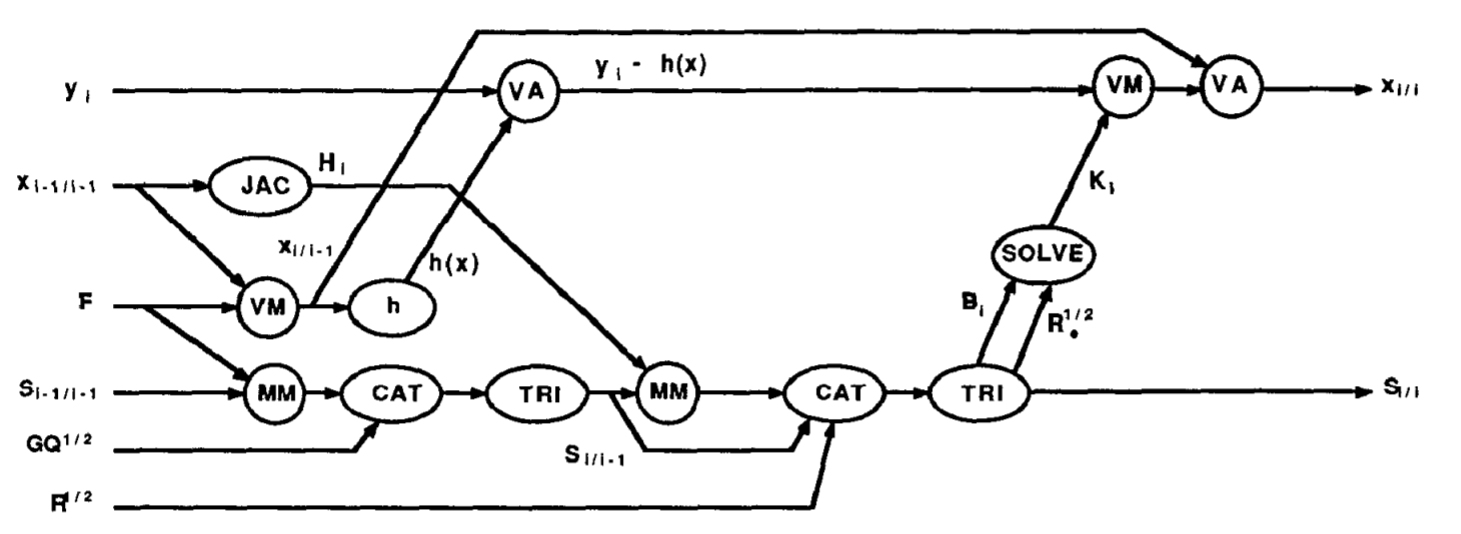
\includegraphics[width=\textwidth]{shaffer.png}
\caption{Dataflow diagram from \cite{Shaffer:1987:IPE:42040.42101}}
\label{fig:shaffer}
\end{figure}

The pipelining of the circuit which was enabled by the removal of recursion from the implementation, resulted in a 360x increase in throughput for the system. This improvement allowed the authors to over 500 targets while collecting 1188 samples/sec.

\subsection{Early Vector Parallelism}
Palis and Krecker, \cite{palis1990parallel}, use the SIMD arrays available in the Connection Machine (a supercomputer manufactured in the late 1980s) to parallelize the work of a single filter and the many-cores of the machine to parallelize the operation of numerous independent filters. The authors use the Square Root Kalman filter which is a variation that allows it to be processed using single-precision calculations without information loss.

The first step to parallelism is to use the SIMD operations to improve the speed of the linear algebra operations. These operations take advantage of the independence of row and elements in matrix operations and can improve the speed of a single Kalman filter operating on a single node. The authors show that the time for computation grows linearly with the number of states in the parallel version rather than cubicly as it does in the serial version. 

Second, the authors demonstrate that when tracking multiple targets the Kalman filters (one or more for each target) can be parallelized by running them on independent processors in the Connection Machine cluster. Their results show that this method can track many more targets than a serial machine.

\section{Modern Implementations and Applications}

\subsection{High Energy Physics}
Cerati et al. have published several similar papers \cite{cerati2015kalman,cerati2016kalman,cerati2015traditional} on parallelizing Kalman filters for use at CERN. The physicists utilize Kalman filters to build tracks of subatomic particles during the runs of the LHC. Given the size and speed at which these events occur, the filtering must occur as rapidly as possible. Similar to Shaffer's work in the 90s, these authors explloit two levels of parallelism on XeonPhi; the vector instructions for the matrix operations and the concurrent bulding of multiple tracks.

For parallelization of linear algebra the authors develop their own library that is optimized for small matrix computation of various architectures. They demonstrate that the use of vector instructions or MICs can produce significant speedup in the application.

The task of parallelizing multiple tracks in this scenario is complicated by the fact that the implementation explores all possible tracks in the case the multiple potential matches are found. This results in a pattern more akin to fork join than map. This problem results in challenges for load balancing since it is unknown which tracks will need to branch. The authors handle this challenge by partitioning in terms of physical region so that threads would track all objects within one part of the beam.


\subsection{Climate Science}
\cite{menard2000assimilation1,menard2000assimilation2,lyster1997parallel}

\subsection{Smart Grid and GPUs}
Recent developments in smart grid technologies have greatly increased the amount and frequency of data available for power grid management. Kalman filters are an important part of the analysis so Karimipour and Dinavahi present a parallelized system based on the kalman filter in \cite{karimipour2015extended}. For this system the authors utilize a machine with a quad-core processor and GPU. To fully utilize available resources they find three types of parallelism seen in figure \ref{fig:mpdse}: Task parallelism between the different equations, data parallelism from the linear algebra, and Linear solver parallelism (for lack of a better phrase) for the parts that aren't in the Kalman filer.

The authors handle the different types of parallelism much like the others did. Linear algebra is sent to GPUs the exploit the SIMD nature of it, while other computations are kept on the CPU. The power grid operations have an interesting twist since they are running additional linear algebra equations at the same time. Additionally, the power grid systems produce between 171 and 23,151 measurements per time step, so the matrices involved are much larger than those in tracking applications allowing the application to take advantage of the wide vectors available in a GPU.


\begin{figure}
\centering
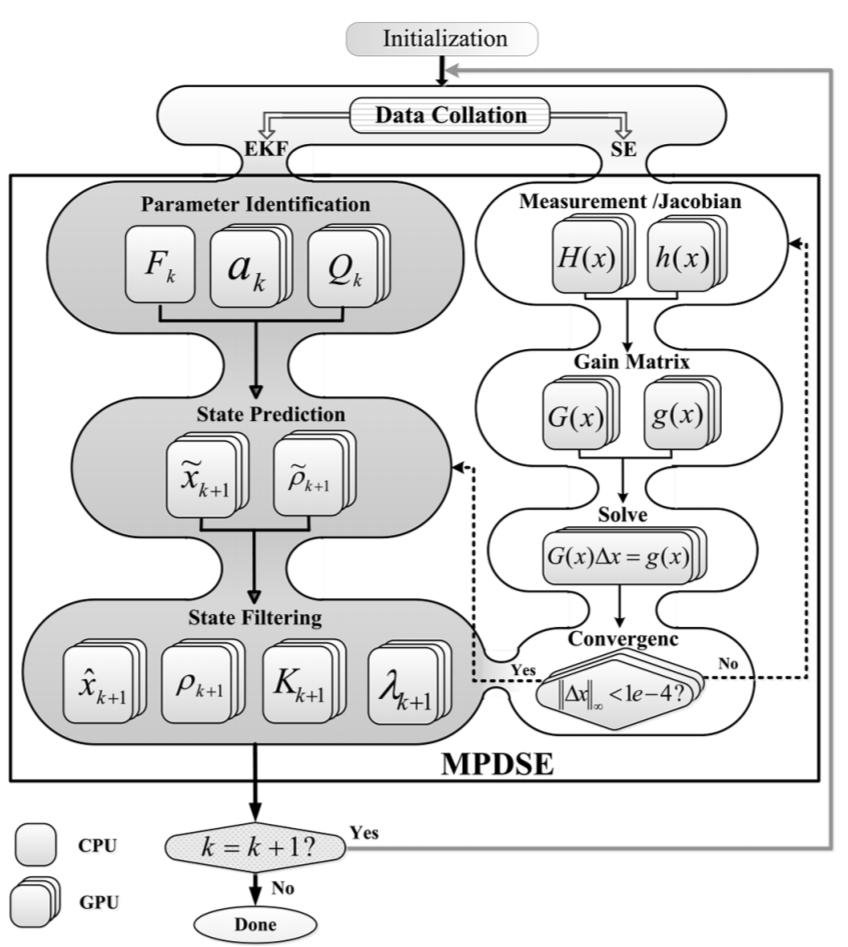
\includegraphics[width=0.5\textwidth]{mpdse.png}
\caption{System flowchart from \cite{karimipour2015extended}}
\label{fig:mpdse}
\end{figure}

\subsection{Cell Tower Power Management}
\cite{rosen2013parallelization}

\section{Sensor Applications}
\cite{rao1991fully,spanos2005distributed,spanos2005approximate,hashemipour1988decentralized}

\section{FPGA Implementations}
While many excellent software applications exist there are also good reasons to implement the Kalman filter using hardware. Two examples,  \cite{bonato2009floating,liu2007efficient}, use FPGA implementations of Kalman filtering to dramatically reduce the time required and the energy used. These implementations employ some level of parallelism but gain further performance benefits by avoiding limitations inherent to software.

Bonato et al. \cite{bonato2009floating}, implement the Extended Kalman filter with the purpose of improving navigation systems for mobile robots.The authors achieve speedup by pipelining the algorithm and ensuring that the most used data (matrix $P$) is the most accessible in the FPGA. Their system has a 3x speedup over a penium processor and consumes 1.3\% of the power. 

Liu et al. \cite{liu2007efficient} apply a similar technique to the Approximate Kalman filter used for feature tracking in computer vision. In this application thousands of features (each with a separate filter) must be tracked at once. The FPGA implementation incorporates enough parallel matrix operation elements that it can perform all or most of the operations simultaneously. Additionally, rather than inverting each matrix the approximate Kalman filter estimates the inversion further minimizing the time.

\section{Conclusion}
Sorry I didn't finish in time. Stay tuned for updates!

\nocite{*}
\bibliographystyle{plain}
\bibliography{filtering}

\end{document}